For each of the main tasks provided in Section \ref{hierarch}, we analyze the
ways in which these tasks could be actualized.

\subsection{Undoing Actions}

For each of the main tasks provided in Section \ref{hierarch}, we analyze the
\begin{figure}[H]
  \centering
  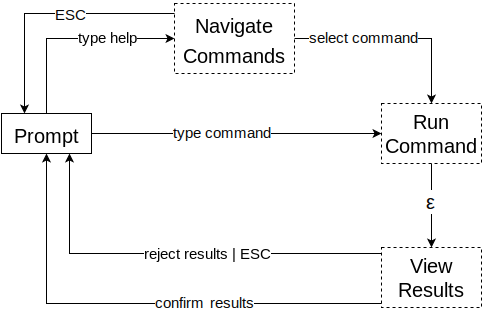
\includegraphics[width=0.8\linewidth]{figures/alternatives/undo_a.png}
  \caption{A breakdown of the procedure for undoing actions.}
  \label{fig:undoa}
\end{figure}

\begin{figure}[H]
  \centering
  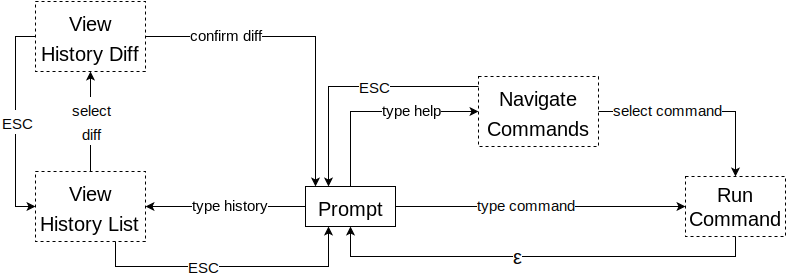
\includegraphics[width=0.8\linewidth]{figures/alternatives/undo_b.png}
  \caption{A breakdown of the procedure for undoing actions.}
  \label{fig:undob}
\end{figure}

\begin{figure}[H]
  \centering
  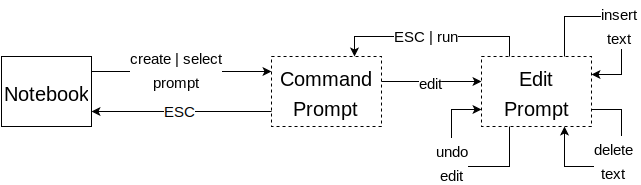
\includegraphics[width=0.8\linewidth]{figures/alternatives/undo_c.png}
  \caption{A breakdown of the procedure for undoing actions.}
  \label{fig:undoc}
\end{figure}

\subsection{Discovery}

\begin{figure}[H]
  \centering
  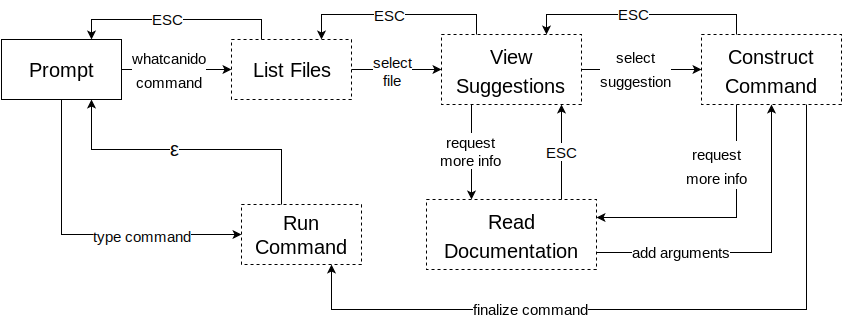
\includegraphics[width=0.8\linewidth]{figures/alternatives/file_a.png}
  \caption{A breakdown of the procedure for undoing actions.}
  \label{fig:undoa}
\end{figure}

\begin{figure}[H]
  \centering
  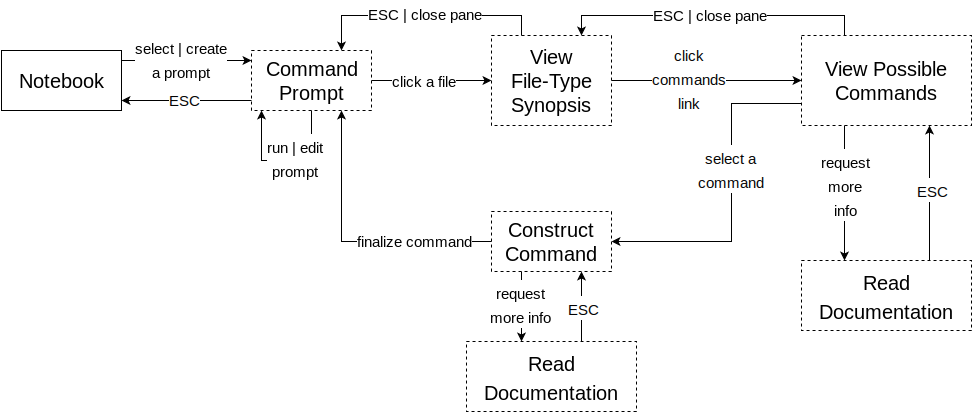
\includegraphics[width=0.8\linewidth]{figures/alternatives/file_b.png}
  \caption{A breakdown of the procedure for undoing actions.}
  \label{fig:undob}
\end{figure}

\begin{figure}[H]
  \centering
  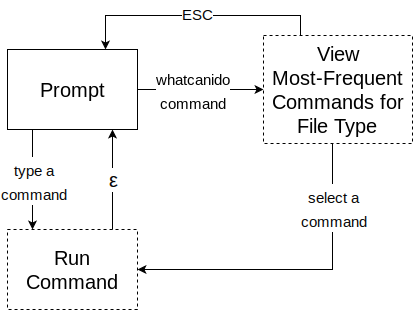
\includegraphics[width=0.8\linewidth]{figures/alternatives/file_c.png}
  \caption{A breakdown of the procedure for undoing actions.}
  \label{fig:undoc}
\end{figure}

\subsection{Workflow Automation}

\begin{figure}[H]
  \centering
  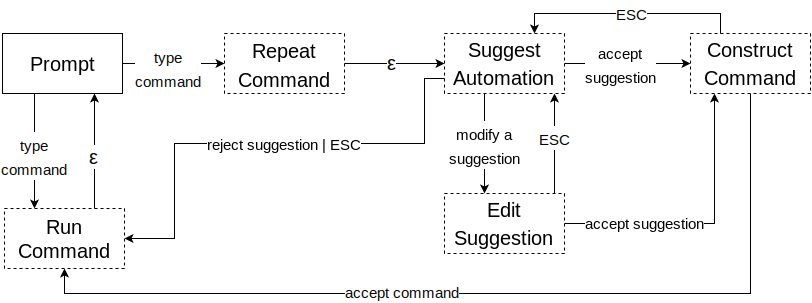
\includegraphics[width=0.8\linewidth]{figures/alternatives/automate_a.png}
  \caption{A breakdown of the procedure for undoing actions.}
  \label{fig:undoa}
\end{figure}

\begin{figure}[H]
  \centering
  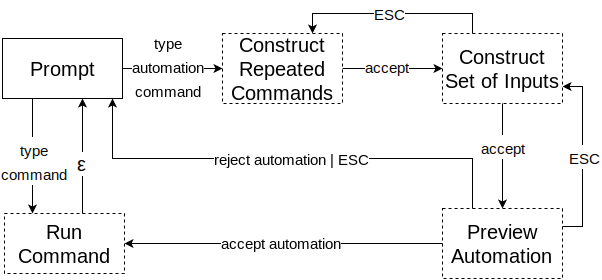
\includegraphics[width=0.8\linewidth]{figures/alternatives/automate_b.png}
  \caption{A breakdown of the procedure for undoing actions.}
  \label{fig:undob}
\end{figure}

\begin{figure}[H]
  \centering
  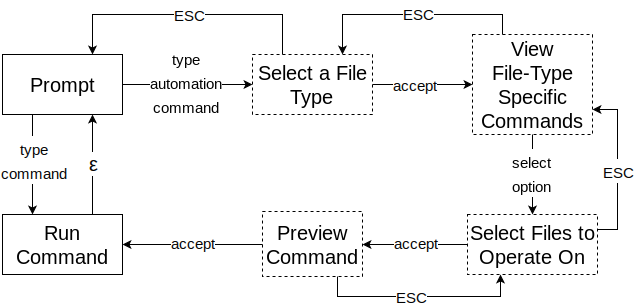
\includegraphics[width=0.8\linewidth]{figures/alternatives/automate_c.png}
  \caption{A breakdown of the procedure for undoing actions.}
  \label{fig:undoc}
\end{figure}

\subsection{Preview Command}

\begin{figure}[H]
  \centering
  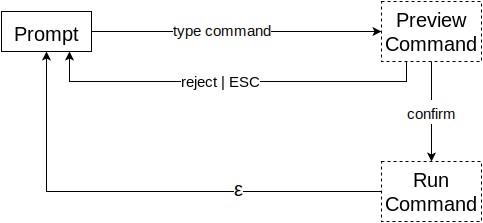
\includegraphics[width=0.8\linewidth]{figures/alternatives/preview_a.png}
  \caption{A breakdown of the procedure for undoing actions.}
  \label{fig:undoa}
\end{figure}

\begin{figure}[H]
  \centering
  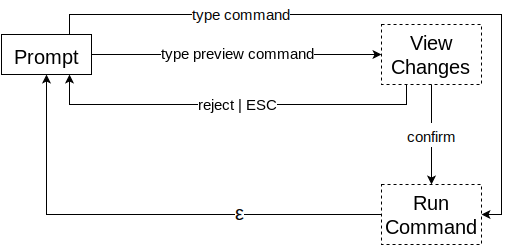
\includegraphics[width=0.8\linewidth]{figures/alternatives/preview_b.png}
  \caption{A breakdown of the procedure for undoing actions.}
  \label{fig:undob}
\end{figure}

\begin{figure}[H]
  \centering
  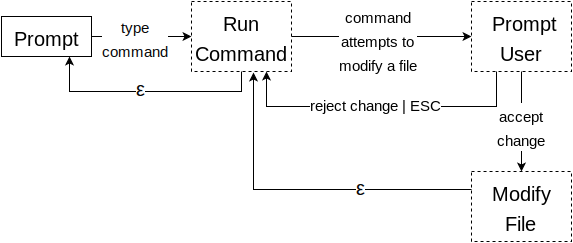
\includegraphics[width=0.8\linewidth]{figures/alternatives/preview_c.png}
  \caption{A breakdown of the procedure for undoing actions.}
  \label{fig:undoc}
\end{figure}
%%% Local Variables:
%%% mode: latex
%%% TeX-master: t
%%% End:
